\documentclass[a4paper]{article}
\usepackage{algorithmicx}
\usepackage{algpseudocode}
\usepackage{graphicx}
\usepackage{vmargin}
\usepackage[utf8]{inputenc}
\usepackage{mdwlist}
\setpapersize{A4}
\setmargins{2.5cm}       % margen izquierdo
{1.5cm}                        % margen superior
{16.5cm}                      % anchura del texto
{23.42cm}                    % altura del texto
{10pt}                           % altura de los encabezados
{1cm}                           % espacio entre el texto y los encabezados
{0pt}                             % altura del pie de página
{2cm}                           % espacio entre el texto y el pie de página
\makeatletter
\setlength{\@fptop}{0pt}
\makeatother
\begin{document}

\section{Ejercicio 3}
\subsection*{a) Explicación de la heuristica}
Antes de explicar la idea vamos a dar algunas definiciones y hacer una aclaración sobre la notación para aportar claridad:
\newline Sea $G = (V, E)$
\newline \textit{\textbf{Def:}} Una \textit{partición parcial} de $G$ va a ser una partición de $G$ a la cual le faltan algunos vértices.
\newline \textit{\textbf{Notación: }} Dada una partición parcial $P$ de $G$, si falta agregar al vértice $u$, entonces $u \notin P$, de lo contrario $u \in P$.
\newline \textit{\textbf{Def:}} Dada una partición parcial $P$ de $G$ y un nodo $u \in V(G)$, decimos que un nodo $v \in V(G)$ es un \textit{par} de $u$ si $(u, v) \in E(G)$ y el peso de la arista $(u, v)$ es máximo sobre los pesos de las aristas $(u, z)$, para los $z \notin P$. $u$ podría no tener ningún par, esto sucede cuando todos sus adyacentes pertenecen a $P$ o directamente no tiene adyacentes.
\newline \textit{\textbf{Def:}} Dada una partición parcial $P$ de $G$ y un nodo $u \in V(G), u \notin P$, la \textit{mejor manera} de agregar a $u$ en $P$ va a ser la que minimice la suma total de los pesos intrapartición de $P$ con los nodos actuales y $u$. Esto también vale para cuando queremos agregar a $u$ y a su par.
\newline
\newline
La idea va a ser ir tomando ciertos nodos del grafo según el valor de una variable $nodoActual$ (que camiará de iteración en interación) e ir ubicándolos de cierta manera en la partición parcial $P$ que vayamos generando. Con respecto al valor de $nodoActual$ vamos a tener dos casos: si efectivamente representa un nodo de $G$, entonces seguro ese nodo va a pertenecer a la partición parcial (de ahora en más $P$) que estamos construyendo; de lo contrario,  $nodoActual$ tendrá un valor indicador (-1) de que no es ningún nodo. 
\newline Si nos encontramos en el primer caso, entonces vamos a tomar (si es posible) un nodo $u \notin P$ adyacente a $nodoActual$ y un nodo $v$ adyacente a $u$, $v$ debe ser un par de $u$. Una vez hecho esto, ubicamos a $u$ y a $v$ en $P$ de la mejor manera. Finalmente, $nodoActual$ pasará a valer $v$ y repetimos lo explicado para este nuevo valor. Si pudimos tomar al nodo $u$ pero no $u$ no tiene par, entonces solo ubicamos a $u$ de la mejor manera y asignamos el valor -1 a $nodoActual$. Más abajo diremos que sucede cuando nos encontramos en el caso en que ni siquiera fue posible encontrar a $u$ (porque $nodoActual$ no tiene adyacentes, todos sus adyacentes ya pertenecen a $P$ o $nodoActual == -1$).
\newline Inicialmente ($P = \{\emptyset_1, \emptyset_2, ..., \emptyset_k\}$) el algoritmo va a tomar (si esto es posible) el par de nodos adyacentes donde el peso de la arista que los une es máximo sobre el peso de cada una de las demás aristas del grafo. En principio, no hay un criterio de elección para cuando existen varios pares de nodos que cumplen esto. Si no existe ningún par de nodos que cumpla esto, entonces no existe ningún par de nodos adyacentes, por lo cual cualquier partición que elijamos va a ser solución. Particularmente el algoritmo generará una partición donde ubique a todos los nodos en un mismo conjunto. En el caso de que sí exista este par de nodos, se procederá a ubicarlos dentro de $P$ de la mejor manera. Una vez hecho esto, si el par de nodos agregados fue $u$ y $v$, el paso siguiente será guardar todos los nodos adyacentes a $v$ en alguna estructura de datos $C$ y elegir como $nodoActual$ a $u$, comenzando así el proceso descripto en el párrafo anterior. Podemos decir ahora, que cuando nos encontramos en el caso en el que $nodoActual$ no tiene adyacentes o directamente no es un nodo, recurriremos a tomar un nodo de $C$.
\newline Si en C no hay ningún nodo que no haya sido agregado $P$ y todavía quedan nodos por agregar a $P$, entonces el algoritmo va a tomar un nodo $u$ de los que faltan (en particular, el de número menor). Si $u$ tiene un par $v$, entonces se procederá a ubicar a $u$ y a $v$ de la mejor manera en $P$ y comenzará el proceso descripto anteriormente con $nodoActual = v$. Si $u$ no tiene par, entonces se ubicará a $u$ de la mejor manera en $P$ y comenzará nuevamente el proceso con $nodoActual = -1$ (porque $u$ no tiene adyacentes no agregados a $P$).
\newline Si $C$ sí tenía algún nodo $u$ que no agregamos $P$, el procedimiento es equivalente: tomar a $u$, si tiene un par $v$ entonces ubicar a $u$ y a $v$ de la mejor manera en $P$ y comenzar de nuevo con $nodoActual = v$, si no tiene par entonces ubicar a $u$ de la mejor manera en $P$ y comenzar de nuevo con $nodoActual = -1$.
\newline Para reforzar la idea, dejamos a continuación un pseudocódigo de alto nivel.
\newline
\begin{algorithmic}[1]
\Procedure{HGolosa}{$G(V, E),\ w: E \rightarrow {\rm I\!R}_+$}
	\State Si $E == \emptyset$ devolver $P = \{V, \emptyset_1, ..., \emptyset_k \}$
	\State Si $k == 1$ devolver $P = \{V\} $
	\newline
	\State $C = \emptyset, P = \emptyset$
	\State Tomar $u_m, v_m \in V$ tales que $(u_m, v_m) \in E \wedge w((u_m, v_m)) \geq w((u, v)) \ \forall u, v \in V, (u, v) \in E$
	\State Insertar a $u_m$ y $v_m$ en conjuntos distintos pertenecientes a $P$
	\State $nodoActual = u_m$
	\State Agregar en $C$ todos los adyacentes a $v_m$
	\newline
	\While{existe algún nodo en V que no esté en P}
		\State $ady \gets -1$
		\If{$nodoActual \neq -1 \wedge tieneAdyacenteNoAgregado(nodoActual, P, G)$}
			\State $ady \gets dameAdyacenteNoAgregado(nodoActual, P, G)$
			\State Agregar en $C$ todos los adyacentes a $nodoActual$ no agregados a $P$
		\Else
			\While{$C \neq \emptyset \wedge (ady == -1 \vee ady \in P)$}
				\State Sacar un nodo $u$ de $C$ y asignarselo a $ady$
			\EndWhile
			\If{$ady == -1 \vee ady \in P$}
				\State $ady \gets dameNoAgregado(G, P)$
			\EndIf
		\EndIf
		\newline
		\If{$tieneAdyacenteNoAgregado(ady, P, G)$}
				\State $par \gets dameParNoAgregado(ady, G, P)$
				\State Agregar $par$ y $ady$ a $P$ de la mejor manera posible
				\State $nodoActual \gets par$
				\State Agregar a $C$, todos los adyacentes de $ady$ que no pertenezcan a $P$
			\Else
				\State Agregar $ady$ a $P$ de la mejor manera posible
				\State $nodoActual \gets -1$
			\EndIf
	\EndWhile
\EndProcedure
\end{algorithmic}
\vspace{0.4cm}
Ya explicado el funcionamiento del algoritmo, es importante destacar que es un algoritmo goloso en \textit{más de un aspecto}. Veamos los distintos tipos de candidatos que considera el algoritmo:
\begin{itemize}
\item Inicialmente, se fija entre todos los pares de nodos adyacentes que hay (estos son sus candidatos), cual es el que tiene un peso máximo en su arista, sobre todas las otras.
\item Cuando toma un nodo $u$ adyacente a $nodoActual$, se fija si puede tomar un nodo $v$ que sea un par de $u$. Los candidatos son todos los adyacentes a $u$ no pertenecientes a $P$.
\item Una vez que tiene a $u$ y a $v$ (o solo a $u$) para agregar a $P$, se va a fijar todas las maneras posibles de agregar ambos (estos son los candidatos) y se va a quedar con la que menos peso haya sumado al peso de $P$ sin estos nodos.
\end{itemize}
Podemos ver que el algoritmo toma una decisión golosa en los tres items anteriores. Es por eso que decimos que es goloso en más de un aspecto.
\vspace{0.4cm}
\subsection*{b) Cálculo del orden de complejidad}
Como queremos analizar el peor caso del algoritmo, vamos a descartar los casos de las líneas 2 y 3, que representan el mejor caso del mismo.
\newline Podemos ver que, en cada iteración el algoritmo agrega a la partición parcial $P$, a lo sumo dos vértices, con lo cual la cantidad total de iteraciones es lineal a la cantidad de nodos, o sea $n$. Para analizar el costo de una iteración, podemos comenzar por ver que, como mínimo, siempre vamos a hacer también una cantidad lineal a $n$ de operaciones. Esto es debido a que el if de la linea 22 siempre se va a ejecutar y, como lo que hace es fijarse si existe algún nodo adyacente a $ady$ no agregado a $P$, no le queda otra que fijarse nodo por nodo a ver si alguno cumple esto. Para entender lo anterior es importante agregar que, en la implementación, trabajamos con matrices de adyacencia y tenemos un arreglo de booleanos, que nos permite saber si un nodo fue agregado a $P$ o no. Por ahora vimos que una iteración es $\Omega(n)$, por lo cual nuestro algoritmo es $\Omega(n^2)$. 
\newline Entre las tantas cosas que faltan considerar, está el costo de agregar el o los nodos a $P$ (líneas 24 y 28). Es fácil ver que el peor caso es cuando hay que agregar dos nodos a $P$ de la mejor manera, y, el hecho de asumir que en un peor caso siempre se agregan dos nodos, no contradice el cáculo que venimos haciendo hasta ahora ya que la cantidad de iteraciones seguiría siendo lineal y el if de la linea 22 es independiente de este hecho. 
\newline \newline Analicemos entonces, el costo de agregar dos nodos $u$ y $v$ en $P$ de la mejor manera: como lo que queremos hacer es minimizar la suma total de los pesos intrapartición, no queda otra que probar todas las combinaciones, es decir:
\begin{enumerate}
\item Calculamos la suma de los pesos de las aristas que unen a $u$ con los vértices de cada conjunto $p_j \in P, j \in [1..k]$ y guardamos esta información en un vector. Cada elemento del vector representa un conjunto de $P$, de manera tal que el vector en una posición contiene el peso que se le agregaría a $P$ si agregáramos a $u$ en ese conjunto.
\item Recorriendo el vector creado en 1. y calculando lo mismo pero para el nodo $v$ (sin necesidad de generar otro vector), nos fijamos cuales son los dos conjuntos de $P$ (podrían ser el mismo) tales que, agregando a $u$ y a $v$ en ellos se minimiza el peso que se le va a sumar al peso anterior de $P$.
\end{enumerate}
\vspace{0.4cm}

Para realizar 1. debemos recorrer los $k$ conjuntos de $P$ y, por cada conjunto sumar el peso determinado por la arista que une a $u$ con cada vértice de ese conjunto. Como no podemos saber cuantos vértices hay en cada conjunto y no hay una manera de acotar esto finamente, vamos a sumar el costo de recorrer los $k$ conjuntos con el costo de calcular las sumas de los pesos de las aristas. Manteniendo el peor caso de agregar 2 elementos en cada iteración, al finalizar el algoritmo el costo total de haber realizado este proceso en cada iteración va a ser:
\[
O(\sum_{i=1}^{n/2}k + 2i) = O(k(n/2)) + O(2\sum_{i=1}^{n/2}i) = O(kn) + O(n^2)
\]

En 2., hacemos algo similar a lo que hacemos en 1. (solo que sin crear un arreglo) pero para el nodo $v$  y, paralelamente vamos recorriendo el arreglo creado en 1. Es decir, por cada vez que calculemos la suma de los pesos de las aristas que unen a $v$ con los nodos de un conjunto particular j (llamémoslo $sumaPesosV_j$), vamos a recorrer (*) el arreglo creado en 1. (que en cada posición tiene un $sumaPesosU_i$) y quedarnos con la suma $sumaPesosV_j + sumaPesosU_i$ más chica.
\newline Siguiendo el mismo razonamiento que antes, el costo de haber realizado este procedimiento en cada iteración del algoritmo, al final estará definido por:
\[
O(\sum_{i=1}^{n/2}k + 2i + k^2) \ \ \ \ (agregamos \ un \ k^2 \ por \ (*))
\]
\[
= O(k(n/2)) + O(2\sum_{i=1}^{n/2}i) + O(k^2(n/2))
\]
\[
= O(kn) + O(n^2) + O(nk^2) = O(n^2) + O(nk^2)
\]

Podemos ver que, como esto tiene una complejidad mayor que la de 1., la complejidad de hacer ambas cosas es $O(n^2) + O(nk^2)$.

\vspace{0.3cm} 
Presentamos a continuación una lista de las operaciones que faltan considerar, con sus respectivas complejidades:
\begin{itemize}
\item La línea 5 es $O(n^2)$ porque requiere recorrer para cada nodo, sus adyacentes y dijimos que utilizamos matrices de adyacencia, con lo cual esto implica recorrer la matriz.
\item La línea 6 es $O(1)$ ya que son dos push\_back en un vectores vacíos dentro de un vector de vectores. Acceder a los vectores vacíos es $O(1)$ ($http://www.cplusplus.com/reference/vector/vector/operator[]/$) y hacer push\_back en vectores vacíos también lo es ya que la complejidad es $O(1)$ amortizada, con lo cual en el peor caso es lineal a la cantidad de elementos y aca esa cantidad es 0 \newline ($http://www.cplusplus.com/reference/vector/vector/push\_back/$).
\item Agregar a $C$ todos los nodos adyacentes a algún nodo (líneas 13, 26). En la implementación, $C$ es una lista de enteros (list$<int>$), donde la complejidad de agregar un elemento al final (que es lo que hacemos) es constante ($http://www.cplusplus.com/reference/list/list/push\_back/$). En el peor caso, vamos a tener que agregar $n$ nodos siempre (un peor caso inalcanzable) y aún así la complejidad final estaría dada por $O(n^2)$ (cantidad lineal de iteraciones por costo de agregar los elementos).
\item Las funciones dameAdyacenteNoAgregado, dameParNoAgregado y tieneAdyacenteNoAgregado, tienen un comportamiento similar. En el peor caso, las tres van a ser $O(n)$ porque van a fijarse todos los adyacentes del nodo (que podrían ser $n - 1$) y, como saber si un nodo fue agregado a $P$ o no es $O(1)$, el costo final es $O(n)$. Como estas funciones son llamadas una cantidad constante de veces dentro del ciclo principal del algoritmo, al finalizar el costo es en el peor caso $O(n^2)$.
\item Tomar un nodo no agregado es $O(n)$ ya que tenemos un arreglo en el que cada posición representa un nodo y el arreglo en esa posición tiene un bool que nos dice si fue o no agregado. Como también se ejecuta una cantidad de veces constante dentro del ciclo principal del algoritmo, el costo total es en el peor caso $O(n^2)$.
\item La guarda del ciclo principal es $O(1)$ ya que en la implementación contamos con un contador que nos dice cuantos nodos fueron agregados a $P$ y, como nunca sacamos un nodo de $P$, basta con evaluar ese contador (que es $O(1)$) para saber si hay que hacer una iteración más o no.
\item El código de las líneas 15, 16 y 17 es $O(n)$ dentro de una iteración. Esto es así porque $C$ no tiene elementos repetidos ya que en la implementación contamos con un arreglo (similar al que nos dice los nodos agregados a $P$) donde cada posición representa un nodo y en esa posición hay un bool que indica si el nodo fue agregado a $C$ o no. Una observación importante para agregar es que, si un nodo $u$ sale de $C$, si no estaba en $P$ seguro se va a agregar inmediatamente, si ya estaba en $C$ entonces simplemente se va a descartar. En ambos casos, $u$ \textbf{no vuelve a entrar a $C$}. Dicho lo anterior, podemos ver que en un peor caso inalcanzable, es costo total de haber ejecutado esta operación en cada iteración es $O(n^2)$.
\item La línea 8 es $O(n)$ ya que en el peor caso, $v_m$ tiene $n - 1$ adyacentes y dijimos que agregar un elemento a $C$ es $O(1)$.
\end{itemize}

\vspace{0.3cm}
Como vemos que las complejidades listadas no superan la complejidad de agregar dos nodos por iteración calculada antes y ya analizamos todas las operaciones que realiza el algoritmo, concluimos que su complejidad es $O(n^2) + O(nk^2)$.
\vspace{0.8cm}
\subsection*{c) Instancias para las cuales la heurística no es buena}
Consideremos un grafo $G_4$ (n = 4, nodos A, B, C y D) donde hay una arista ($A, B$) de peso máximo y todas las demás aristas tiene peso estrictamente menor. Pensemos al grafo como un $K_4$ sin una arista, de manera tal que los nodos $A$ y $B$ estén conectados a los nodos $C$ y $D$ pero estos dos últimos no sean adyacentes entre sí.
\newline Observemos la figura que está a continuación y muestra exactamente como sería este grafo con algunos pesos elegidos de manera no arbitraria.
\begin{figure}[h]
\centering
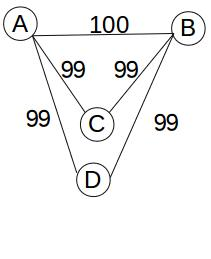
\includegraphics[scale=0.8]{grafoHGolosaMala1.jpg}\caption{$G_4$}
\end{figure}
\pagebreak

Pensemos como trabajaría el algoritmo con $G_4$ y con $k = 2$: inicialmente tomaría la arista ($A, B$) por ser la (única) que tiene peso máximo, ubicando así a $A$ y $B$ en conjuntos distintos de $P$. Luego, trabajaría con $A$ o con $B$. Sin pérdida de generalidad, supongamos que trabaja con $B$ y encola los adyacentes de $A$ que no están en $P$ (o sea $C$ y $D$). Ahora va a elegir un adyacente a $B$ para meter en la partición, supongamos que elige a $C$ (nuevamente, no perdemos generalidad porque si eligiera a $D$ sucedería lo mismo al final). Ubicar a $C$ de la mejor manera posible en $P$ significa probar de todas las maneras y quedarse con la mejor, pero solo hay dos maneras (porque $K = 2$) y ambas suman lo mismo: 99. Dado que resta ubicar a $D$, es fácil ver que, como $C$ y $D$ no son adyacentes pero $C$ sí es adyacente a $B$ y $A$, va a suceder lo mismo. Es decir, de cualquier manera que ubiquemos a $D$, el peso que se le va a agregar a $P$ va a ser 99. Esto concluye que cualquier orden que elija el algoritmo para tomar los nodos, la suma va a ser siempre (en este caso) 198.
\newline Claramente no es la forma óptima de ubicar los nodos en $P$, ya que si hubieramos ubicado a $A$ y $B$ en un mismo conjunto de $P$ y a $C$ y $D$ en el otro conjunto, la suma sería 100.
\newline
\newline Podríamos generalizar este caso para que el algoritmo sea arbitrariamente malo cuando $k = 2$. Para lograr esto, simplemente agregamos más nodos y los conectamos únicamente con $A$ y $B$.
\begin{figure}[h]
\centering
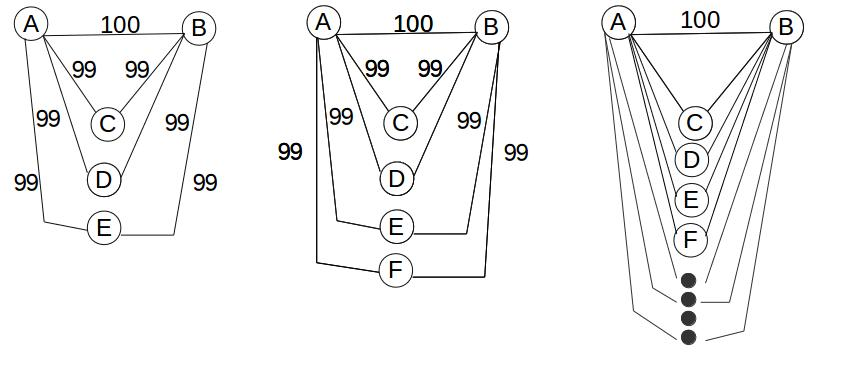
\includegraphics[scale=0.5]{grafoHGolosaMala3.jpg}
\end{figure}
\pagebreak

Los primeros dos grafos son $G_4$ con uno ($E$) y dos nodos más ($E$ y $F$), respetando siempre la manera de conectar vértices (por cada vértice agregado, éste debe ser adyacente necesaria y únicamente a $A$ y $B$). El tercer ejemplo describe que podríamos seguir agregando vértices hacia abajo que respeten las adyacencias necesarias (no pusimos los pesos de las demás aristas por una cuestión de espacio), agrandando más y más la brecha entre la suma de la partición óptima y la que devuelve la heurística. Entonces, para toda esta clase de grafos (y no solo para el ejemplo particular de $G_4$) el algortimo es malo, ya que siempre va a elegir la arista de peso máximo, separando así sus extremos en conjuntos distintos. En estos grafos, hacer eso constituye una mala decisión, porque luego por cada nodo que se agregue, \textit{siempre} se va a estar sumando 99, cuando en realidad, la suma óptima siempre es 100.
\newline Es importante ver también que, los pesos 100 y 99 fueron elegidos con la intención de hacer evidente el problema, pero podrían ser otros y podrían no ser valores tan cercanos. Incluso, no es necesario que, para los nodos $T$ distintos de $A$ y $B$, se cumpla que el peso de ($A, T$) sea igual al peso de ($B, T$). La restricción en cuanto a los pesos que se debe cumplir para que el algoritmo no de la solución óptima, es que dados dos nodos distintos de $A$ y $B$, llamemoslos $C$ y $D$, sea cierto que $w((A, C)) + w((B, D)) > w((A, B)) \ \wedge \ w((A, D)) + w((B, C)) > w((A, B)).$ Si eso sucede, y el grafo es uno de la clase que describimos antes, entonces seguro la heurística no da la solución óptima.

\end{document}